
\chapter{A NetGen-compatible map browser}

This is a tool allowing to display various kind of maps and to represent 
locations of interest such as sensors set in the country. 
As this tool is developped on the same platform as NetGen, the procedures described 
in chapter \ref{sec:chapter1} will apply to access the software: 
\begin{itemize}
\item start a fresh image and ensure that the NetGen package is loaded with one of the last 
version (1.28.1.2.5 should work)
\item open the store dialog from VisualWorks main window
\item select GoogleMap package (we need to change this name)
\item select version 1.15.5.2 or later, and type load from the pop-up menu
\end{itemize}

The initial window displays as show figure \ref{fig:initialGmap}. 

\begin{figure}
\begin{center} 
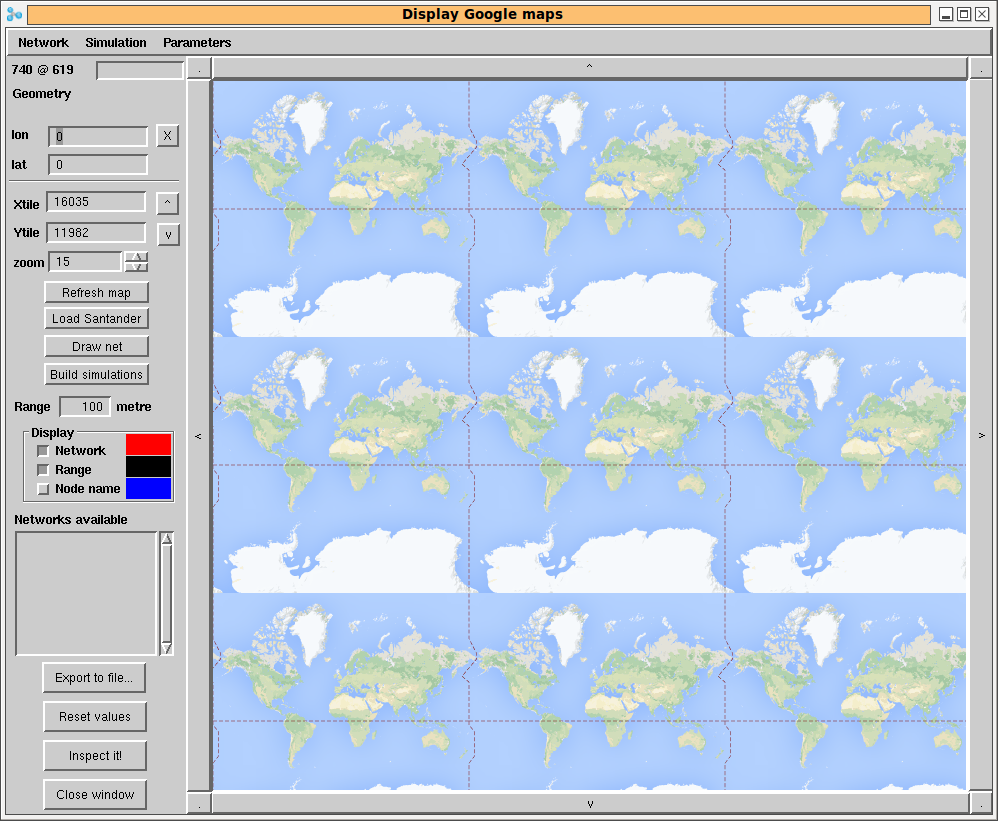
\includegraphics[width=8cm]{gmap.png}
\caption{Initial view on the map browser: the right part displays tiles from the map 
from public servers. The left column displays geographic information and allows 
to control network presentation. }
\label{fig:initialGmap}
\end{center}
\end{figure}


Be fore developing actual programs for wireless sensor networks, it
is good to check if the cooperation of local programs will lead
to working and efficient results.

The distributed behaviour comes from:

\begin{itemize}
\item an architecture specification, such as {\tt mekong1.occ},
\item a behaviour executed by nodes, such as {\tt nodes-test-include.occ}.
\end{itemize}

The two descriptions are orthogonal, meaning that one can make
evolution on the architecture at fixed behaviour, or make evolutions on
the behaviour with fixed architecture. The situation is well known
in computer architecture. It is named an Y methodological approach,
and was popularized by Gajski.
The bottom branch carrying measures produced from tools (energy, 
response time, cost, etc\ldots).

Simulation is a key method to take measures on complex situations.
To use simultation, we need to reproduce real dispersion of behaviours,
and random number generators are useful for this.

\section{Random numbers in Occam}

The Occam {\tt course} library provides the random function that
has two parameters and provides a result as a couple of numbers
(integers).

The small program {randomSample.occ}  demonstrates the general use for random.

\begin{lstlisting}  
#USE "course.lib"
-- montre le fonctionnement du generateur aleatoire.
PROC Random(CHAN OF BYTE in,out,err)
  VAL INT N IS 5: 
  VAL INT K IS 10:  -- borne de tirage de random : [0,K[
  PROC Genere(VAL INT seedInitial)
    INT x,seed:
    SEQ
      x,seed:=random(K,seedInitial)
      SEQ i=0 FOR N
        SEQ
          x,seed:=random(K,seed)
          out.number(x,2,out)
          out.string("*n",0,out)
      out.string("___",0,out)
      out.string("*n",0,out)
  :
  
  SEQ
    Genere(12)
    Genere(2)
    Genere(12) -- la souche est la meme que le premier cas et donne le meme tirage.
:
\end{lstlisting}

Compiling ({\tt kroc -lcourse randomSample.occ}), and executing  ({\tt ./randomSample})produces the 
following trace:
\begin{lstlisting}./randomSample
 1
 3
 1
 8
 0
___
 8
 9
 6
 3
 4
___
 1
 3
 1
 8
 0
___
\end{lstlisting}

It is noticeable that the seed value allows to reproduce exactly the same random sequence of numbers.
Thus, if we are to use this mechanism inside network simulators, we must vary the seed at each node.
The unique  {\tt Identity} of nodes is a good way to do this.
